% CS 7050 Term Project — Final Report
% Kay Rand Morgan, Section W01
\documentclass[10pt,letterpaper]{article}
\usepackage[T1]{fontenc}
\usepackage[utf8]{inputenc}
\usepackage[scaled=0.95]{helvet}
\usepackage{courier}
\usepackage[margin=0.95in,top=0.85in,bottom=0.85in]{geometry}
\usepackage[table]{xcolor}
\usepackage{titlesec}
\usepackage{booktabs}
\usepackage{tabularx}
\usepackage{array}
\usepackage{enumitem}
\usepackage{microtype}
\usepackage{graphicx}
\usepackage{float}
\usepackage{multirow}
\usepackage[font=small,labelfont={bf,color=accent},skip=4pt]{caption}
\usepackage{tikz}
\usetikzlibrary{positioning,arrows.meta,shapes.multipart,fit,calc}
\usepackage[colorlinks=true,urlcolor=accent,linkcolor=accent,citecolor=accent]{hyperref}

\definecolor{accent}{HTML}{2E4D7B}
\definecolor{rowhead}{HTML}{EDF1F7}
\definecolor{rule}{HTML}{B9C4D4}
\definecolor{factfill}{HTML}{DCE7F5}
\definecolor{aggfill}{HTML}{FBE3D6}
\definecolor{dimfill}{HTML}{F4F6F9}
\definecolor{pend}{HTML}{B4400F}

\renewcommand{\familydefault}{\sfdefault}
\titleformat{\section}{\normalfont\large\bfseries\color{accent}}{\thesection.}{0.5em}{}
\titleformat{\subsection}{\normalfont\normalsize\bfseries\color{accent}}{\thesubsection}{0.5em}{}
\titlespacing*{\section}{0pt}{9pt}{3pt}
\titlespacing*{\subsection}{0pt}{6pt}{2pt}
\setlist[itemize]{leftmargin=1.2em,topsep=1pt,itemsep=1pt,parsep=0pt}
\setlist[enumerate]{leftmargin=1.4em,topsep=1pt,itemsep=1pt,parsep=0pt}
\setlength{\parskip}{3.5pt}
\setlength{\parindent}{0pt}
\setlength{\emergencystretch}{3em}
\renewcommand{\arraystretch}{1.12}
\renewcommand{\tt}[1]{\texttt{#1}}
\newcommand{\pending}{{\color{pend}\itshape pending NRP run}}
\pagestyle{plain}

\begin{document}

{\color{black!70}\small CS 7050 --- Data Warehousing and Data Mining}\\[2pt]
{\color{accent}\LARGE\bfseries Term Project Report}\\[3pt]
{\color{black!70}\small Kennesaw State University $\cdot$ College of Computing and Software Engineering}

\vspace{3pt}
{\color{rule}\hrule height 0.6pt}
\vspace{7pt}

\begin{tabularx}{\textwidth}{|>{\columncolor{rowhead}\bfseries\small}p{1.5in}|X|}
\hline
Name & Kay Rand Morgan \\ \hline
Section & W01 \\ \hline
Project title & From Clickstream to Early Alert: A Dimensional Warehouse and Mining Pipeline for Virtual Learning Environment Engagement Data \\ \hline
Code & \url{https://github.com/kayrandmorgan-oss/cs7050-oulad-early-alert} \\ \hline
Date & October 18, 2026 \\ \hline
\end{tabularx}

\vspace{6pt}
\fcolorbox{rule}{rowhead}{\parbox{\dimexpr\textwidth-2\fboxsep-2\fboxrule}{\small
\textbf{Summary.} The 10.66M-row OULAD clickstream and its six companion tables were loaded into a MySQL~8
fact constellation: two facts, six conformed dimensions, and two materialized aggregates. The warehouse rebuilds
from the raw CSVs with one command in 12 minutes and passes 28 of 28 reconciliation checks. In particular, all
39,605,099 clicks reach the fact table. An 11-query OLAP pack returns identical results from the base fact and
the aggregates, and the aggregates answer 7 of the queries up to \textbf{688$\times$} faster. From a week-4
feature view with a machine-verified no-leakage cutoff, logistic regression predicts fail/withdraw for students
still enrolled on day~28. On held-out October presentations it reaches \textbf{ROC-AUC 0.719}, which is
\textbf{+8.1} accuracy points over the majority class. At a threshold tuned on training data it recalls
\textbf{80\%} of at-risk students. The result is modest, and it is reported as modest. $k$-means finds four
engagement archetypes whose fail/withdraw rates range from 29\% to 65\%. The disparate-impact audit passes the
four-fifths screen for gender, deprivation (IMD) and disability, but not for age band. Given a schema
context generated from the live warehouse, an open 7B code model answers \textbf{47.5\%} of 40 held-out analyst
questions exactly and chooses the aggregate tables for 91\% of eligible questions. Without that context it
answers none. The LoRA condition is packaged for the course GPU hub.}}

%======================================================================
\section{Problem and research question}
Virtual learning environments (VLEs) log every click, but in tables built to run courses rather than to analyze
them. This project builds both halves of CS~7050 on one public dataset. The first half is a warehouse that answers
coordinator questions in seconds, such as ``how does week-by-week engagement in this module compare with the same
module last term, by activity type?''. The second half is an early-alert mining layer trained on feature marts
drawn from that warehouse. The research question, unchanged from the proposal, is: \emph{using only VLE
interaction and registration data observable through the first four weeks of a presentation, and excluding
protected attributes, how accurately can final outcome (pass/distinction vs.\ fail/withdrawn) be predicted, and
what engagement archetypes exist?} Week~4 is chosen because an alert at that point can still be acted on.
Published accuracy figures on this dataset that use whole-course features are leaky for this purpose.

%======================================================================
\section{Data and profiling}
\textbf{Source.} The data is the Open University Learning Analytics Dataset (OULAD) [1], CC~BY~4.0: 22 module
presentations of 7 modules (2013--2014; ``B'' = February start, ``J'' = October start). In October 2026 the
official download link redirected to a page without the archive. The CSVs were therefore taken from a public
mirror, and the 8-part \tt{studentVle} was reassembled. Every row count matches the dataset paper
(Table~\ref{tab:src}), and the reconciliation suite (Section~\ref{sec:etl}) checks the files end to end. An
independent second mirror had the same clickstream row count but capped \tt{sum\_click} at 6, so it was rejected
as a cleaned derivative.

\begin{table}[H]\centering\small
\caption{Source tables and profiling highlights (\tt{etl/profile\_raw.py}, \tt{out/profile\_report.json}).}\label{tab:src}
\begin{tabular}{@{}lrp{4.3in}@{}}
\toprule
\textbf{Table} & \textbf{Rows} & \textbf{Profiling findings} \\ \midrule
\tt{studentVle} & 10,655,280 & days $-25$..269; 2,195,960 rows repeat a (student, site, day) key; max 6,977 clicks; 39,605,099 clicks total \\
\tt{studentAssessment} & 173,912 & 173 NULL scores; 1,909 banked; 2,057 submitted before day 0 \\
\tt{studentInfo} & 32,593 & 28,785 distinct students; \tt{imd\_band} NULL ×1,111 and \tt{`10-20'} missing its \% ×3,516; \tt{age\_band} varies for 72 students \\
\tt{studentRegistration} & 32,593 & 45 NULL registration dates; 5,040 unregistered before day 28; 93 Withdrawn without a date \\
\tt{vle} & 6,364 & 20 activity types; \tt{week\_from/to} 82\% NULL (not used) \\
\tt{assessments} & 206 & 11 exams with no date \\
\tt{courses} & 22 & lengths 234--269 days \\
\bottomrule
\end{tabular}
\end{table}
Each anomaly has a documented decision (D1--D14 in \tt{etl/DECISIONS.md}). The four that most shape the results:
\begin{itemize}
\item \textbf{D8.} Repeated (student, site, day) rows are \emph{summed}, not dropped. They are separate
interaction records. Dropping them would lose 20\% of rows and break the click-total reconciliation.
\item \textbf{D9.} Zero-activity rows are generated only inside a student's \emph{registered span}, so a student
who has left is not padded with fake inactivity.
\item \textbf{D13.} The 5,040 enrollments that unregistered before day~28 stay in the warehouse but leave the
modeling population. An alert cannot help a student who has already left, and keeping them would inflate accuracy
with trivially easy cases.
\item \textbf{D14} (found by the OLAP pack, not the profiler). In BBB, CCC and DDD, 97--100\% of computer-marked
assessments (CMAs) are ``submitted'' 2--3 days after their listed date. In FFF and GGG, all CMAs share one
end-of-module date. Lateness is therefore interpreted for tutor-marked assessments (TMAs) only.
\end{itemize}

%======================================================================
\section{Warehouse design}
\textbf{Conceptual model.} Figure~\ref{fig:er} shows the source ER model. \tt{studentInfo} and
\tt{studentRegistration} share the composite key (module, presentation, student). \tt{studentVle} and
\tt{studentAssessment} are the two event streams. They sit at different grains: daily site clicks, and one row per
submitted assessment.

\begin{figure}[H]\centering
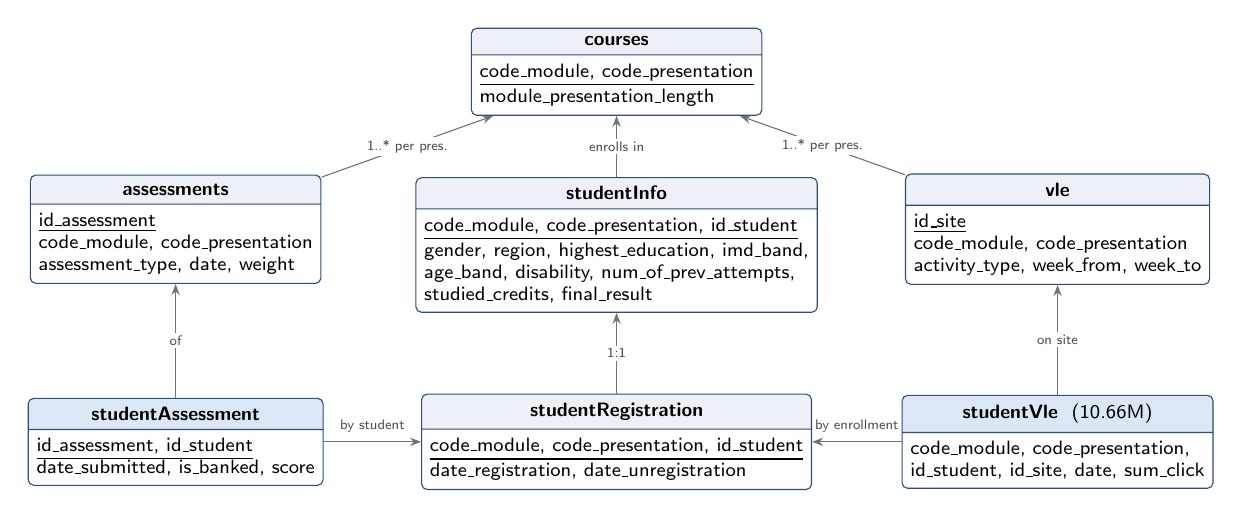
\begin{tikzpicture}[
  ent/.style={draw=accent,rounded corners=2pt,font=\scriptsize,align=left,inner sep=3pt,
              rectangle split,rectangle split parts=2,rectangle split part fill={rowhead,white}},
  ev/.style={ent,rectangle split part fill={factfill,white}},
  rel/.style={-{Stealth[length=4pt]},draw=black!55,thin},
  lab/.style={font=\tiny,fill=white,inner sep=1pt,text=black!70}]
\node[ent] (courses) at (0,0) {\textbf{courses}\nodepart{two}\underline{code\_module, code\_presentation}\\ module\_presentation\_length};
\node[ent] (asm) at (-5.6,-2.0) {\textbf{assessments}\nodepart{two}\underline{id\_assessment}\\ code\_module, code\_presentation\\ assessment\_type, date, weight};
\node[ent] (vle) at (5.6,-2.0) {\textbf{vle}\nodepart{two}\underline{id\_site}\\ code\_module, code\_presentation\\ activity\_type, week\_from, week\_to};
\node[ent] (info) at (0,-2.2) {\textbf{studentInfo}\nodepart{two}\underline{code\_module, code\_presentation, id\_student}\\ gender, region, highest\_education, imd\_band,\\ age\_band, disability, num\_of\_prev\_attempts,\\ studied\_credits, final\_result};
\node[ent] (reg) at (0,-4.7) {\textbf{studentRegistration}\nodepart{two}\underline{code\_module, code\_presentation, id\_student}\\ date\_registration, date\_unregistration};
\node[ev] (sa) at (-5.6,-4.7) {\textbf{studentAssessment}\nodepart{two}\underline{id\_assessment, id\_student}\\ date\_submitted, is\_banked, score};
\node[ev] (sv) at (5.6,-4.7) {\textbf{studentVle} \ (10.66M)\nodepart{two}code\_module, code\_presentation,\\ id\_student, id\_site, date, sum\_click};
\draw[rel] (asm) -- node[lab]{1..* per pres.} (courses);
\draw[rel] (vle) -- node[lab]{1..* per pres.} (courses);
\draw[rel] (info) -- node[lab]{enrolls in} (courses);
\draw[rel] (reg) -- node[lab]{1:1} (info);
\draw[rel] (sa) -- node[lab]{of} (asm);
\draw[rel] (sa.east) -- node[above,font=\tiny,text=black!70]{by student} (reg.west);
\draw[rel] (sv) -- node[lab]{on site} (vle);
\draw[rel] (sv.west) -- node[above,font=\tiny,text=black!70]{by enrollment} (reg.east);
\end{tikzpicture}
\caption{Conceptual ER model of the seven OULAD source tables (event streams shaded). Underlined attributes are keys.}\label{fig:er}
\end{figure}

\textbf{Dimensional model.} The source becomes a fact constellation of two facts that share conformed dimensions
(Figure~\ref{fig:star}), following Kimball's four-step method [3]. Every dimension uses integer surrogate keys, and
natural keys are kept as degenerate attributes.

\begin{figure}[H]\centering
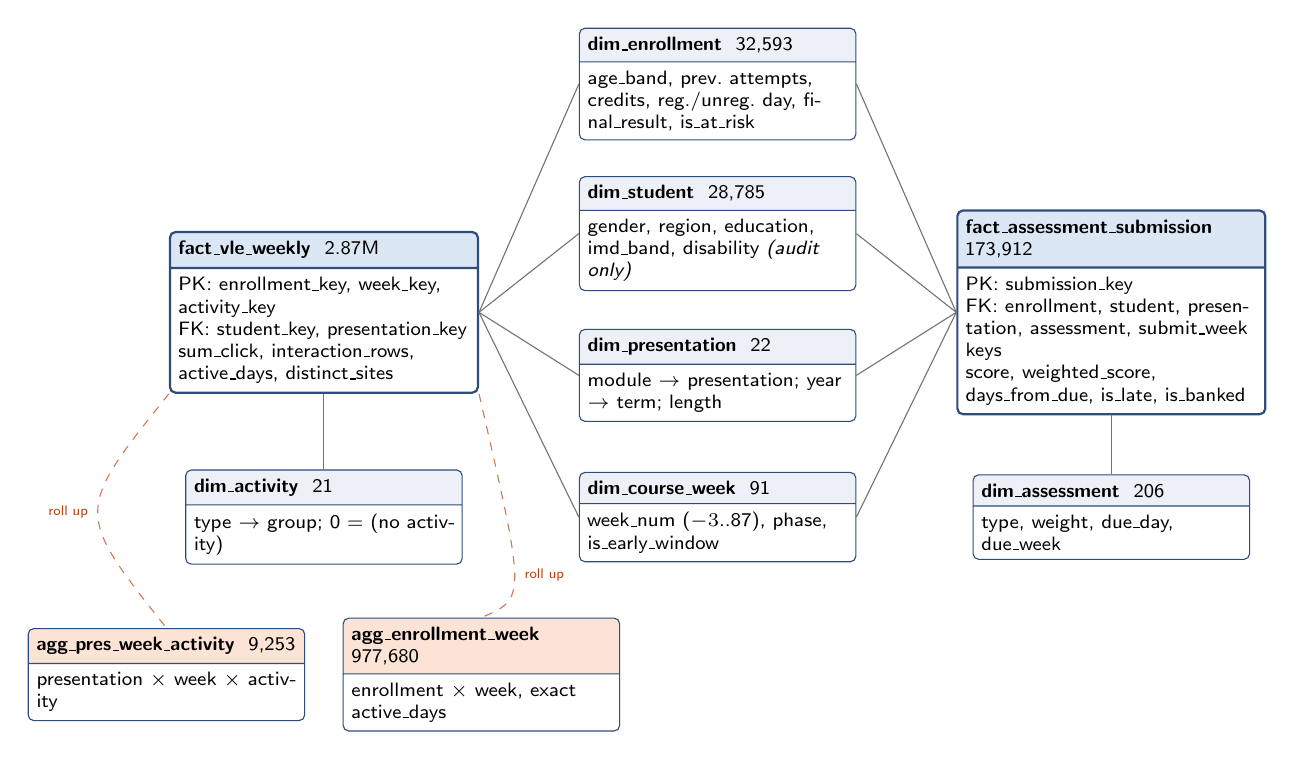
\begin{tikzpicture}[
  dim/.style={draw=accent,rounded corners=2pt,font=\scriptsize,align=left,inner sep=3pt,text width=3.3cm,
              rectangle split,rectangle split parts=2,rectangle split part fill={rowhead,white}},
  fact/.style={dim,rectangle split part fill={factfill,white},text width=3.7cm,line width=0.8pt},
  agg/.style={dim,rectangle split part fill={aggfill,white},text width=3.3cm},
  fk/.style={draw=black!55,thin}]
\node[fact] (f1) at (-5.0,0) {\textbf{fact\_vle\_weekly}\ \ 2.87M\nodepart{two}PK: enrollment\_key, week\_key, activity\_key\\ FK: student\_key, presentation\_key\\ sum\_click, interaction\_rows,\\ active\_days, distinct\_sites};
\node[fact] (f2) at (5.0,0) {\textbf{fact\_assessment\_submission}\ \ 173,912\nodepart{two}PK: submission\_key\\ FK: enrollment, student, presentation, assessment, submit\_week keys\\ score, weighted\_score, days\_from\_due, is\_late, is\_banked};
\node[dim] (enr) at (0,2.9) {\textbf{dim\_enrollment}\ \ 32,593\nodepart{two}age\_band, prev.\ attempts, credits, reg./unreg.\ day, final\_result, is\_at\_risk};
\node[dim] (stu) at (0,1.0) {\textbf{dim\_student}\ \ 28,785\nodepart{two}gender, region, education, imd\_band, disability \emph{(audit only)}};
\node[dim] (pres) at (0,-0.8) {\textbf{dim\_presentation}\ \ 22\nodepart{two}module $\rightarrow$ presentation; year $\rightarrow$ term; length};
\node[dim] (wk) at (0,-2.6) {\textbf{dim\_course\_week}\ \ 91\nodepart{two}week\_num ($-3$..87), phase, is\_early\_window};
\node[dim] (act) at (-5.0,-2.6) {\textbf{dim\_activity}\ \ 21\nodepart{two}type $\rightarrow$ group; 0 = (no activity)};
\node[dim] (asmd) at (5.0,-2.6) {\textbf{dim\_assessment}\ \ 206\nodepart{two}type, weight, due\_day, due\_week};
\node[agg] (a1) at (-7.0,-4.6) {\textbf{agg\_pres\_week\_activity}\ \ 9,253\nodepart{two}presentation $\times$ week $\times$ activity};
\node[agg] (a2) at (-3.0,-4.6) {\textbf{agg\_enrollment\_week}\ \ 977,680\nodepart{two}enrollment $\times$ week, exact active\_days};
\foreach \d in {enr,stu,pres,wk} {\draw[fk] (f1.east) -- (\d.west); \draw[fk] (f2.west) -- (\d.east);}
\draw[fk] (f1) -- (act); \draw[fk] (f2) -- (asmd);
\draw[fk,dashed,draw=pend!70] (f1.south west) .. controls +(-1.2,-1.5) .. node[left,font=\tiny,text=pend]{roll up} (a1.north);
\draw[fk,dashed,draw=pend!70] (f1.south east) .. controls +(0.6,-2.6) .. node[right,font=\tiny,text=pend]{roll up} (a2.north);
\end{tikzpicture}
\caption{The fact constellation: two facts (blue), six conformed dimensions, and two materialized aggregates (orange). Row counts are after the load.}\label{fig:star}
\end{figure}

\textbf{Grain decisions.}
\begin{itemize}
\item \textbf{Weekly rather than daily.} Daily grain would reproduce the 10.66M-row source. Weekly grain matches
the alert cadence and cuts the clickstream to 2.52M clicked rows.
\item \textbf{Relative course week, not calendar date.} \tt{week\_num = FLOOR(day/7)+1}, so week~1 is days 0--6
and weeks $\le 0$ are pre-start. This makes presentations of different lengths and start dates directly comparable.
\item \textbf{\tt{activity\_type} as a dimension, not 20 pivoted columns.} This refines the proposal's grain
statement. Fact~1 is one row per \emph{enrollment $\times$ course week $\times$ activity type with clicks}, plus
exactly one \tt{(no activity)} row (\tt{activity\_key}~0) for each registered enrollment-week with no clicks
(350,649 rows). ``Clicked nothing in week~3'' becomes a countable fact without multiplying zero rows by 20 types.
\tt{sum\_click} is fully additive. \tt{active\_days} is additive across weeks but not across activity types,
which is why the aggregate \tt{agg\_enrollment\_week} computes it exactly from staging.
\item \textbf{\tt{age\_band} on the enrollment, other demographics on the student.} \tt{age\_band} changes
between presentations for 72 students. Gender, region, education, IMD and disability never change, so they are
Type-1 attributes of \tt{dim\_student}.
\end{itemize}
Table comments hold each table's grain statement. The text-to-SQL prompt (Section~\ref{sec:llm}) reads these
comments from \tt{information\_schema}.

%======================================================================
\section{ETL and reconciliation}\label{sec:etl}
\tt{etl/build\_warehouse.py} drops and rebuilds the database in three layers.
\begin{enumerate}
\item \textbf{Staging.} The CSVs are loaded as-is with \tt{pandas} and \tt{SQLAlchemy}. The clickstream is loaded
in 200k-row chunks. The proposal's \tt{LOAD DATA INFILE} fallback is kept behind \tt{--load-data} but was not
needed.
\item \textbf{Transform and load.} The 17 timed SQL steps in \tt{sql/transform\_load.sql} cover surrogate-key
assignment with \tt{ROW\_NUMBER()}, the cleaning decisions, zero-row generation, the aggregates, and foreign keys
added after the bulk load.
\item \textbf{Reconciliation.} 28 assertions must all pass, or the build exits non-zero and nothing downstream
runs.
\end{enumerate}

\begin{table}[H]\centering\small
\caption{Build timings (2 vCPU, 8 GB, MySQL 8.0.46; \tt{out/build\_log\_initial\_run.json}).}\label{tab:build}
\begin{tabular}{@{}lr@{\hspace{2.5em}}lr@{}}
\toprule
\textbf{Step} & \textbf{s} & \textbf{Step} & \textbf{s} \\ \midrule
Stage 10.66M clicks (chunked pandas) & 267.2 & Zero-activity rows (fact + A2) & 21.7 \\
Fact 1, clicked rows (GROUP BY) & 130.8 & A1 \tt{agg\_pres\_week\_activity} & 11.9 \\
A2 \tt{agg\_enrollment\_week} & 95.7 & Foreign keys on facts & 63.3 \\
Dimensions (6) & 17.8 & Reconciliation (28 checks) + DB setup & 94.6 \\
\midrule
\multicolumn{3}{@{}l}{\textbf{Total, raw CSVs $\rightarrow$ verified warehouse}} & \textbf{723.8} \\
\bottomrule
\end{tabular}
\end{table}

\begin{table}[H]\centering\small
\caption{Reconciliation suite (selected; all 28 pass). R00 checks compare against the CSV files themselves.}\label{tab:recon}
\begin{tabular}{@{}llrr@{}}
\toprule
& \textbf{Assertion} & \textbf{Expected} & \textbf{Actual} \\ \midrule
R00 & \tt{studentVle.csv} click total = fact clicks & 39,605,099 & 39,605,099 \\
R02 & Fact interaction rows = clickstream rows & 10,655,280 & 10,655,280 \\
R03 & \tt{dim\_student} = distinct students in \tt{studentInfo} & 28,785 & 28,785 \\
R04/R05 & Enrollments / submissions preserved & 32,593 / 173,912 & 32,593 / 173,912 \\
R06 & SUM(score) preserved & 13,169,342 & 13,169,342 \\
R07/R08 & Both aggregates sum to the fact & 39,605,099 & 39,605,099 \\
R09 & Presentations whose clicks disagree with staging & 0 & 0 \\
R13 & Enrollment-weeks with both a zero row and clicks & 0 & 0 \\
R16 & At-risk label = Fail + Withdrawn count & 17,208 & 17,208 \\
\bottomrule
\end{tabular}
\end{table}

\textbf{End-to-end rebuild test (M5).} The warehouse was dropped and rebuilt from the raw CSVs a second time. That
run took 718.9~s and again passed 28 of 28 checks. The leakage check and all model results were then regenerated
and are identical to the first run.

%======================================================================
\section{OLAP}
\tt{olap/olap\_queries.sql} contains 11 queries covering the operations promised in the proposal.
\tt{olap/run\_olap.py} runs every variant once to warm up and then five timed runs, and reports the median. Where
an aggregate can answer the question, it asserts that the aggregate variant returns exactly the same rows as the
base-fact variant.

\begin{table}[H]\centering\small
\caption{OLAP query pack: median runtimes, base fact vs.\ materialized aggregate (\tt{out/olap\_runtimes.csv}). All 7 aggregate variants return identical rows.}\label{tab:olap}
\begin{tabular}{@{}llp{2.9in}rrr@{}}
\toprule
& \textbf{Operation} & \textbf{Question} & \textbf{Base ms} & \textbf{Agg ms} & \textbf{Speed-up} \\ \midrule
Q01 & roll-up & Clicks by module $\rightarrow$ presentation, \tt{WITH ROLLUP} & 7,460 & 10.8 & 688$\times$ \\
Q02 & drill-down & FFF: clicks/student by presentation $\rightarrow$ phase & 6,288 & 10.8 & 584$\times$ \\
Q03 & slice & BBB-2014J: clicks and users by activity group & 364 & --- & --- \\
Q04 & dice & BBB, FFF $\times$ Oct $\times$ weeks 1--4 $\times$ 2 groups $\times$ outcome & 236 & --- & --- \\
Q05 & pivot & Activity type $\times$ week 1--10 matrix, DDD-2014J & 298 & 1.9 & 160$\times$ \\
Q06 & cross-tab & Final outcome $\times$ week-1--4 engagement decile & 2,745 & 859 & 3.2$\times$ \\
Q07 & cross-term & CCC 2014B vs.\ 2014J, weekly clicks/student & 339 & 5.2 & 65$\times$ \\
Q08 & roll-up (hier.) & Activity group $\rightarrow$ type, by outcome & 8,935 & --- & --- \\
Q09 & roll-up (fact 2) & Mean score, \% late by module $\rightarrow$ assessment type & 357 & --- & --- \\
Q10 & drill-across & Engagement (fact 1) beside scores (fact 2) per presentation & 6,731 & 332 & 20$\times$ \\
Q11 & zero-activity & \% of registered students with no clicks, weeks 1--8 & 1,034 & 756 & 1.4$\times$ \\
\bottomrule
\end{tabular}
\end{table}

\textbf{Aggregate navigation.} The speed-up tracks how much the aggregate shrinks the scan. A1 (9,253 rows) is
310 times smaller than the fact, and queries that only need presentation, week and activity run two to three
orders of magnitude faster. A2 is only 2.9 times smaller, and its gain on per-student questions (Q06, Q11) is a
modest 1.4--3.2$\times$. Questions that split clicks by an enrollment attribute together with an activity
attribute (Q04, Q08) cannot use either aggregate. For those questions the base fact remains necessary.

\begin{figure}[H]\centering
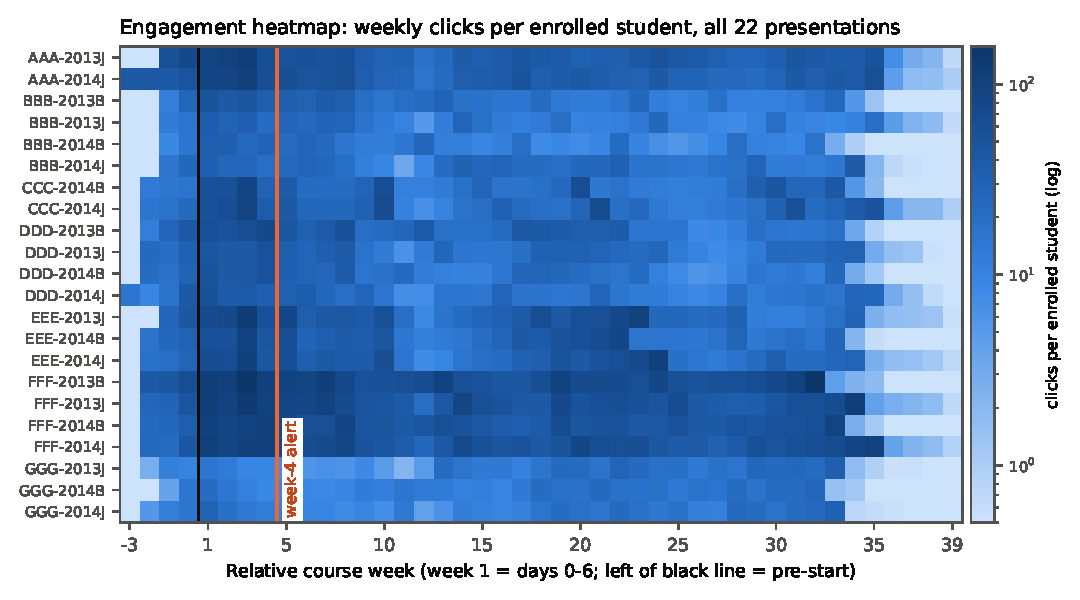
\includegraphics[width=\textwidth]{../figures/engagement_heatmap.pdf}
\caption{Weekly clicks per enrolled student (A1 aggregate). Every presentation shows a pre-start ramp, peak
intensity in the early weeks, sustained mid-course activity, and a sharp drop after its final week (weeks
34--39). FFF and AAA run at roughly 3$\times$ the per-student intensity of BBB and GGG.}\label{fig:heat}
\end{figure}

\textbf{What the cube shows.} Engagement in the first four weeks is strongly ordered against outcome (Q06,
Figure~\ref{fig:dec}). The bottom decile has no week-1--4 clicks at all, and 97\% of that decile fails or
withdraws. In the top decile 25\% do. Already in week~1, 28\% of eventual fail/withdraw students who are still
registered have zero clicks, against 13\% of eventual passers (Q11). By week~8 that gap widens to 42\% vs.\ 14\%.
The coordinator's motivating question is answered by Q07. CCC's October 2014 cohort engaged more per student
than its February cohort in every one of weeks 1--10 (by 2--21\%, most in week~4), then less in weeks 11--12. Q10 drills across the two
facts. Per-student clicks and mean scores alone do not order presentations by risk: GGG has the lowest
engagement but also one of the lowest at-risk rates (38--43\%). That is the first sign that \emph{relative},
within-presentation engagement matters more than raw volume, and the models confirm it.

\begin{figure}[H]\centering
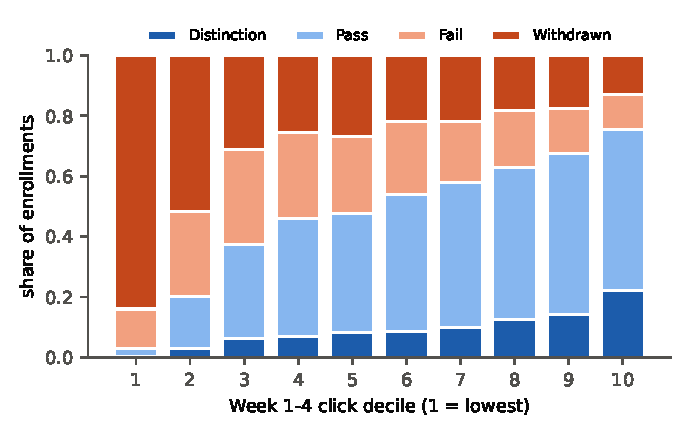
\includegraphics[width=0.56\textwidth]{../figures/outcome_by_decile.pdf}
\caption{Final outcome by week-1--4 click decile, all 32,593 enrollments (Q06).}\label{fig:dec}
\end{figure}

%======================================================================
\section{Mining}
\subsection{Feature mart and leakage control}
\tt{v\_features\_week4} (\tt{sql/feature\_mart.sql}) defines the modeling population and features.
\begin{itemize}
\item \textbf{Population.} Every enrollment still registered on day~28: 27,553 rows, 44.2\% at risk.
\item \textbf{Features (29).} Registration attributes: prior attempts, studied credits, registration day, and a
missing-date flag. Pre-start clicks and active days. Clicks in each of weeks 1--4. Active days, active weeks and
last active week in weeks 1--4. Distinct sites in week~4. Clicks per activity group and number of activity types
used. Two derived features: clicks relative to the presentation median, and a week-4 vs.\ week-1 trend. Module
indicators.
\item \textbf{What the view cannot see.} The label, the unregistration date, any assessment data, and every
protected attribute. Protected attributes are reachable only through a separate audit view.
\end{itemize}
The cutoff is enforced in SQL by joining only weeks with \tt{is\_early\_window = 1}, meaning
\tt{last\_day $\le$ 27}. \tt{mining/check\_leakage.py} asserts it independently. The script recomputes all 16
clickstream features from the \emph{raw CSV} with pandas using only days $< 28$, and they match the SQL view for
all 27,553 enrollments. It then repeats the computation with no cutoff, which is what a leaky pipeline would
produce, and gets 25,679 mismatches. That shows the test can detect leakage when it is present. Finally, it checks
the model's feature list against a forbidden-column list. The result was \textbf{LEAKAGE CHECK PASS}.

\subsection{Classification}
Three models were compared against a majority-class baseline:
\begin{itemize}
\item \textbf{Logistic regression (LR).} Standardized features, log-transformed counts, and $C$ chosen by inner
3-fold CV.
\item \textbf{CART decision tree.} Raw counts, with depth and leaf size chosen by inner CV.
\item \textbf{Gaussian naive Bayes (NB).} Log-transformed counts.
\end{itemize}
Two validation designs were used. The first is 5-fold stratified CV over all presentations. The second, which
matters for deployment, trains on the 10,647 February-start enrollments and tests on the 16,906 October-start
enrollments. The decision threshold is never left at 0.5. It is tuned on the \emph{training} out-of-fold
probabilities to maximize recall subject to a precision floor of 0.60, then applied unchanged to the test set. The
floor reflects the cost asymmetry: an unnecessary check-in costs an advisor minutes, while a missed student may
cost a course.

\begin{table}[H]\centering\small
\caption{5-fold stratified CV, all presentations (mean $\pm$ s.d., threshold 0.5).}\label{tab:cv}
\begin{tabular}{@{}lcccccc@{}}
\toprule
\textbf{Model} & \textbf{Accuracy} & \textbf{Precision} & \textbf{Recall} & \textbf{F1} & \textbf{ROC-AUC} & \textbf{Brier} \\ \midrule
Majority baseline & .558 $\pm$ .000 & --- & .000 & .000 & .500 & .442 \\
Logistic regression & \textbf{.673 $\pm$ .003} & \textbf{.662 $\pm$ .005} & \textbf{.530 $\pm$ .010} & \textbf{.589 $\pm$ .006} & \textbf{.724 $\pm$ .008} & \textbf{.208} \\
Decision tree (CART) & .652 $\pm$ .003 & .634 $\pm$ .010 & .505 $\pm$ .039 & .561 $\pm$ .022 & .689 $\pm$ .009 & .218 \\
Naive Bayes & .646 $\pm$ .005 & .646 $\pm$ .017 & .443 $\pm$ .032 & .525 $\pm$ .019 & .692 $\pm$ .009 & .318 \\
\bottomrule
\end{tabular}
\end{table}

\begin{table}[H]\centering\small
\caption{Presentation-held-out test (train February $\rightarrow$ test October; test base rate 41.3\%).}\label{tab:ho}
\begin{tabular}{@{}l c ccc c cccc@{}}
\toprule
& & \multicolumn{3}{c}{\textbf{Threshold 0.5}} & & \multicolumn{4}{c}{\textbf{Tuned threshold (precision floor 0.60 on train)}} \\
\cmidrule(lr){3-5}\cmidrule(l){7-10}
\textbf{Model} & \textbf{AUC} & \textbf{Acc.} & \textbf{Prec.} & \textbf{Recall} & \textbf{$t$} & \textbf{Prec.} & \textbf{Recall} & \textbf{F1} & \textbf{Flagged} \\ \midrule
Majority baseline & .500 & .587 & --- & .000 & --- & --- & --- & --- & --- \\
Logistic regression & \textbf{.719} & \textbf{.668} & .593 & .622 & .392 & .519 & \textbf{.801} & \textbf{.630} & 63.7\% \\
Decision tree (CART) & .679 & .643 & .562 & .612 & .426 & .501 & .761 & .604 & 62.6\% \\
Naive Bayes & .692 & .652 & .628 & .382 & .001 & .523 & .734 & .611 & 57.9\% \\
\bottomrule
\end{tabular}
\end{table}

\begin{figure}[H]\centering
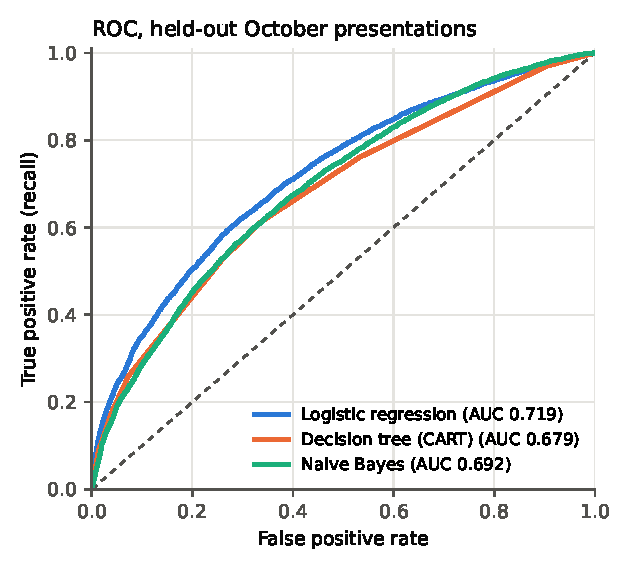
\includegraphics[width=0.325\textwidth]{../figures/roc_holdout.pdf}\hfill
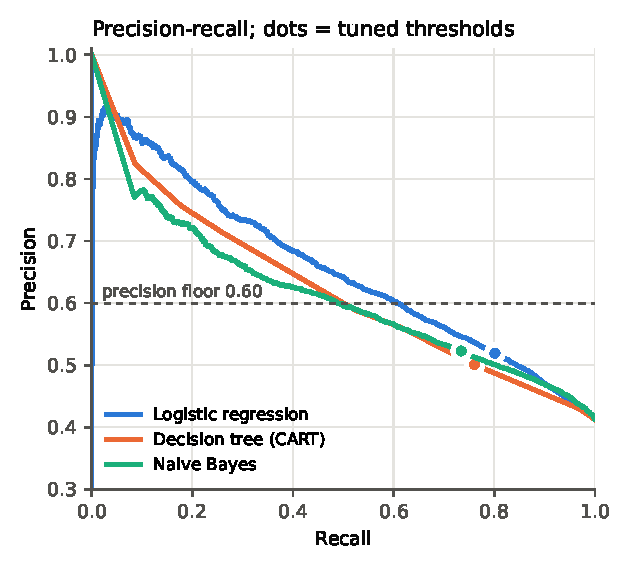
\includegraphics[width=0.325\textwidth]{../figures/pr_holdout.pdf}\hfill
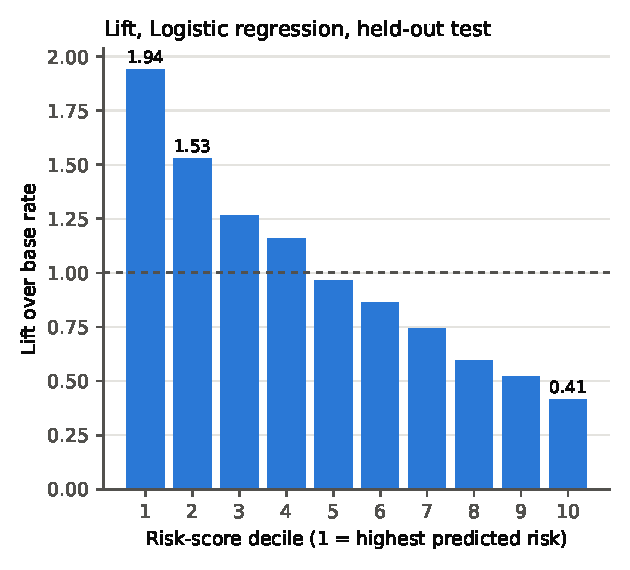
\includegraphics[width=0.325\textwidth]{../figures/lift_holdout.pdf}
\caption{Held-out October test. Left: ROC curves. Centre: precision--recall curves, with dots marking the tuned
operating points. Right: lift by risk decile for logistic regression.}\label{fig:roc}
\end{figure}

\textbf{Reading the results.} Logistic regression is the best model on every summary metric in both validation
designs. On the held-out October presentations it beats the majority class by \textbf{8.1 accuracy points} (66.8\%
vs.\ 58.7\%) with AUC 0.719. Its top risk decile is 80.0\% at-risk, a lift of 1.94, and the top three deciles
contain 47\% of all at-risk students. These numbers are modest, and that is the honest result of removing leakage.
Four weeks of clicks separate students only moderately well. Three further findings matter for deployment.
\begin{itemize}
\item \textbf{Prior shift between cohorts.} The at-risk rate is 48.8\% in February presentations and 41.3\% in
October ones. A threshold that gives 0.60 precision on February data gives 0.52 on October data. The floor is
therefore a training-time promise, not a guarantee. Table~\ref{tab:sens} gives the operating menu an advisor
would actually choose from.
\item \textbf{Robustness.} A second split, 2013 $\rightarrow$ 2014, gives AUCs of 0.705 (LR), 0.677 (CART) and
0.691 (NB), with the same ranking. Weka~3.6 on the same Feb/Oct ARFF files reproduces the results
(\tt{mining/weka\_crosscheck.sh}): Logistic AUC 0.717 (vs.\ 0.719), J48 0.685 (vs.\ CART 0.679), and NaiveBayes
0.682 on untransformed counts (vs.\ 0.692 on log counts).
\item \textbf{Naive Bayes behaves as predicted.} The nine log-click features have a mean absolute pairwise
correlation of 0.57, and 7 of 36 pairs exceed 0.7. NB therefore double-counts the same evidence. Its ranking (AUC)
stays competitive, but its probabilities are badly calibrated (Brier 0.320 vs.\ 0.212), so its tuned threshold
collapses to 0.001. NB is usable as a ranker but not as a probability.
\end{itemize}

\begin{table}[H]\centering\small
\caption{Operating-point menu for logistic regression: thresholds chosen on training out-of-fold probabilities, evaluated on the October test.}\label{tab:sens}
\begin{tabular}{@{}cccccc@{}}
\toprule
\textbf{Precision floor (train)} & \textbf{Threshold} & \textbf{Test precision} & \textbf{Test recall} & \textbf{Test F1} & \textbf{Students flagged} \\ \midrule
0.55 & .312 & .468 & .905 & .617 & 79.7\% \\
\textbf{0.60} & \textbf{.392} & \textbf{.519} & \textbf{.801} & \textbf{.630} & \textbf{63.7\%} \\
0.65 & .461 & .565 & .688 & .620 & 50.3\% \\
0.70 & .540 & .620 & .549 & .582 & 36.5\% \\
\bottomrule
\end{tabular}
\end{table}

\textbf{Interpretability.} The CART grid search chose depth~3, and 93\% of its split importance is on one feature:
week-1--4 clicks \emph{relative to the presentation median}. The depth-3 tree reads as three alert rules:
\begin{itemize}
\item Below the presentation median by more than about 30\% (log-ratio $\le -0.34$): flag.
\item Near the median but active in at most 3 of the 4 weeks: flag.
\item Above the median: do not flag.
\end{itemize}
Logistic regression tells the same story with more nuance. The largest standardized coefficients that reduce risk
are active days (--0.25), relative clicks (--0.20), last active week (--0.17), week-2 clicks (--0.13) and
pre-start clicks (--0.13). Two features increase risk: prior attempts (+0.11), and navigation-only (homepage)
clicks (+0.12), which can be read as logging in without opening content. Module effects are as large as any
behavior (GGG --0.31, BBB --0.20, DDD +0.17). Note that module AAA has no February presentation, so the
held-out model never saw it. An early version also included raw total clicks, which made the LR coefficients
collinear (+1.19 total vs.\ --1.11 relative). It was removed for interpretability, and AUC was unchanged
(0.716 $\rightarrow$ 0.719).

\subsection{Clustering: engagement archetypes}
$k$-means ($n_\mathrm{init}=10$) was run for $k=2..10$ on nine standardized week-1--4 features: log clicks for the
pre-start period and each of weeks 1--4, active days, assessment and communication shares, and activity types.
Outcomes were not inputs. Mean silhouette peaks at $k=2$ (0.306), but $k=2$ is only a high/low volume split. The
elbow is at $k=4$: within-cluster SS falls 15\% from 3 to 4 clusters and only 7\% from 4 to 5, while silhouette
holds at 0.248 before dropping to 0.195 at $k=5$. $k=4$ was therefore chosen. Ward hierarchical clustering on a
stratified sample of 4,000 enrollments, cut at 4, agrees with $k$-means at adjusted Rand index \textbf{0.64}. For
comparison the ARI is 0.22 at $k=2$, so the four-cluster structure is the more reproducible one.

\begin{figure}[H]\centering
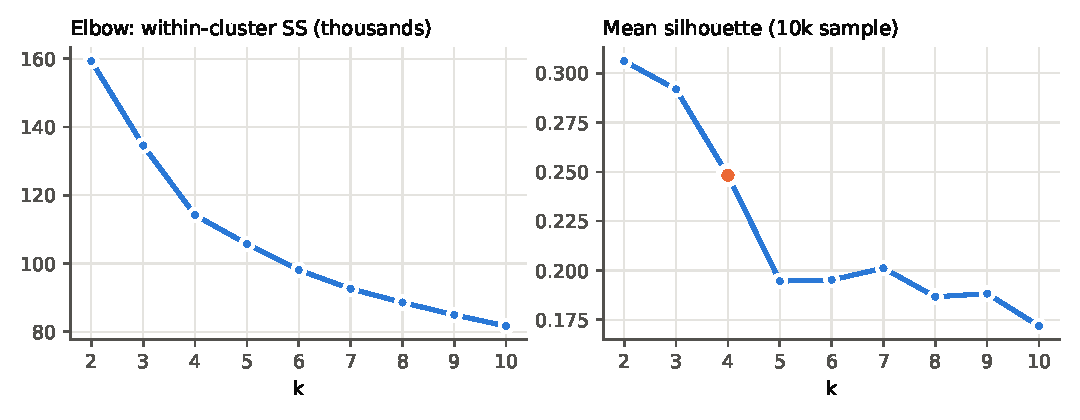
\includegraphics[width=0.72\textwidth]{../figures/kmeans_elbow_silhouette.pdf}\\[4pt]
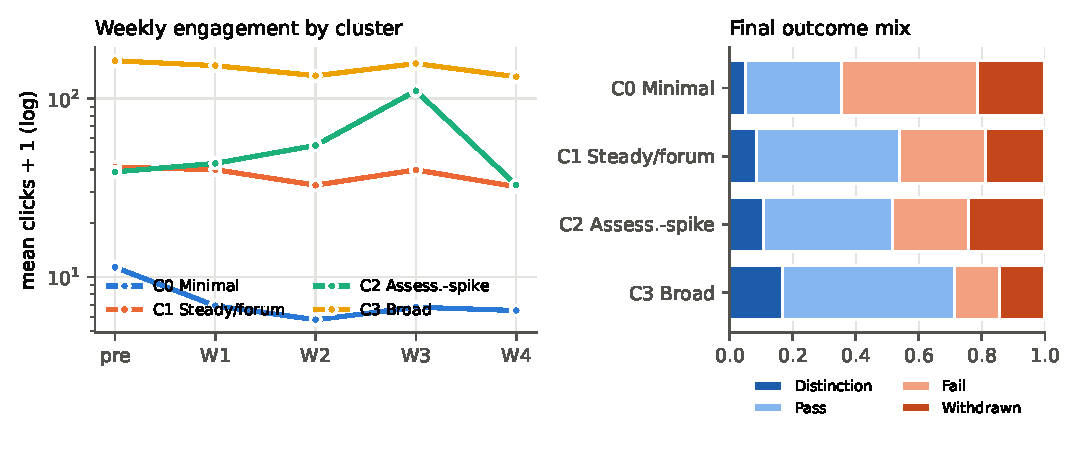
\includegraphics[width=0.82\textwidth]{../figures/cluster_profiles.pdf}
\caption{Top: model selection. Bottom: mean weekly clicks per cluster (log scale) and final-outcome mix.}\label{fig:clu}
\end{figure}

\begin{table}[H]\centering\small
\caption{Engagement archetypes, $k=4$ (27,553 enrollments still registered at week 4; \tt{out/cluster\_profiles.csv}).}\label{tab:clu}
\begin{tabular}{@{}p{3.1cm}rrrrrrr@{}}
\toprule
\textbf{Archetype} & \textbf{Share} & \textbf{Median clicks} & \textbf{Active days} & \textbf{Assess.\ share} & \textbf{Forum share} & \textbf{Withdrawn} & \textbf{At risk} \\ \midrule
C0 Minimal presence & 19.6\% & 14 & 2.2 & 1\% & 7\% & 21.4\% & \textbf{64.6\%} \\
C1 Steady, forum-engaged & 32.2\% & 120 & 8.4 & 2\% & 31\% & 18.7\% & 46.1\% \\
C2 Assessment-spike & 14.7\% & 205 & 8.8 & 54\% & 7\% & \textbf{24.3\%} & 48.2\% \\
C3 Broad and consistent & 33.5\% & 466 & 18.6 & 11\% & 33\% & 14.4\% & \textbf{28.6\%} \\
\bottomrule
\end{tabular}
\end{table}
The archetypes are substantive, not just volume bands. C2 averages only about 32--54 clicks in weeks 1, 2 and~4,
then spikes to 109 in week~3 when the first quiz/CMA falls due, and 54\% of its clicks are on assessment
activities. It is the ``assessment-only'' pattern the proposal anticipated, and it has the highest withdrawal rate
(24\%) despite higher volume than C1. The proposal's hypothetical ``front-loaded then absent'' archetype did
\emph{not} emerge as a cluster in weeks 1--4. Those students are spread across C0 and C1, and separating them
would need later weeks, which the alert cutoff excludes. Of the C0 students who were still registered at week~4,
65\% go on to fail or withdraw. That makes C0 the obvious first call list. C3 has the highest distinction rate
(16.7\%).

\subsection{Disparate-impact audit}
After prediction, the October test predictions of the deployed model (LR at $t=0.392$) were joined to the
protected attributes and summarized in aggregate (\tt{mining/audit.py}; Table~\ref{tab:audit}). For each group the
audit reports how often students are flagged, how often they are truly at risk, and the recall and false-positive
rate. The screen applied is the four-fifths rule on flag rate: lowest group divided by highest, among groups with
$n \ge 100$.

\begin{table}[H]\centering\small
\caption{Disparate-impact audit, held-out October test (16,906 enrollments).}\label{tab:audit}
\begin{tabular}{@{}llrrrrrr@{}}
\toprule
\textbf{Attribute} & \textbf{Group} & \textbf{n} & \textbf{Actual at-risk} & \textbf{Flag rate} & \textbf{Precision} & \textbf{Recall} & \textbf{FPR} \\ \midrule
\multirow{2}{*}{Gender} & F & 7,492 & .397 & .622 & .494 & .775 & .522 \\
 & M & 9,414 & .425 & .648 & .539 & .821 & .520 \\ \midrule
\multirow{3}{*}{Age band} & 0--35 & 11,685 & .430 & .678 & .523 & .825 & .567 \\
 & 35--55 & 5,076 & .375 & .548 & .508 & .743 & .431 \\
 & 55+ & 145 & .303 & .407 & .492 & .659 & .297 \\ \midrule
\multirow{5}{*}{IMD quintile} & 0--20\% (most deprived) & 3,278 & .508 & .656 & .614 & .793 & .515 \\
 & 20--40\% & 3,603 & .445 & .646 & .557 & .809 & .516 \\
 & 40--60\% & 3,374 & .407 & .637 & .509 & .797 & .527 \\
 & 60--80\% & 3,155 & .375 & .631 & .485 & .815 & .521 \\
 & 80--100\% (least) & 2,879 & .337 & .627 & .435 & .808 & .535 \\ \midrule
\multirow{2}{*}{Disability} & N & 15,328 & .401 & .634 & .508 & .802 & .522 \\
 & Y & 1,578 & .520 & .658 & .629 & .795 & .509 \\
\bottomrule
\end{tabular}
\end{table}

\textbf{Findings, reported whatever they show.}
\begin{itemize}
\item \textbf{Gender and disability} pass comfortably: flag-rate ratios of 0.96 and 0.96, recall gaps of at most
4.7 points, and FPR gaps under 1.4 points.
\item \textbf{Age band fails the screen.} The flag-rate ratio is 0.60, driven by the small 55+ group. Even
between 0--35 and 35--55 the ratio is 0.81, right at the line. Younger students are flagged more, and their
false-positive rate is 13.6 points higher than the 35--55 group (0.567 vs.\ 0.431). Their actual risk is also
higher, but the model over-flags them relative to that risk (flag/actual 1.58 vs.\ 1.46).
\item \textbf{IMD reveals a subtler pattern.} Flag rates are almost flat (0.63--0.66, ratio 0.83, passing the
screen) even though actual risk falls from 51\% to 34\% across quintiles. Recall is equal across groups. The
consequence is that a flag means less for affluent students (precision 0.44) than for deprived ones (0.61).
Because the model never sees IMD, it cannot reproduce that gradient. Whether that is the desired form of fairness
is a policy decision rather than a modeling one.
\end{itemize}
Any deployment should monitor the age-band FPR gap, and should present a flag as an invitation to check in, never
as a judgment.

%======================================================================
\section{LLM component: natural-language queries over the warehouse}\label{sec:llm}
\textbf{Design.} An open-weight code model writes MySQL for 40 held-out analyst questions. The gold SQL comes from
the OLAP pack and variants of it (\tt{text2sql/questions\_test.py}). Each question states the columns it expects,
so ``same rows'' is well defined. Matching is order- and column-order-insensitive, with numbers compared at two
decimals. 22 questions can be answered exactly from an aggregate table, and they define the
\emph{aggregate-navigation rate}. The three conditions are:
\begin{itemize}
\item \textbf{No schema.} The model gets only the dialect and the question.
\item \textbf{Schema in prompt.} The context is built \emph{programmatically from the live warehouse}
(script \tt{schema\_context.py}): compact DDL with keys and foreign keys for the 10 dimension, fact and
aggregate tables, each table's grain statement read back from its comment, and a data dictionary of every
low-cardinality value. With the instructions, the prompt is 2,438 tokens. Staging tables are deliberately excluded.
\item \textbf{LoRA + schema.} The same prompt, after LoRA fine-tuning [5] on 200 (question, SQL) pairs. The pairs
come from 21 parameterized templates (\tt{text2sql/make\_train\_pairs.py}). Each pair was executed and checked to
return rows, and none duplicates a test question or its gold SQL.
\end{itemize}

\textbf{What ran where.} The proposal's degradation path was used for the prompt-only conditions.
Qwen2.5-Coder-7B-Instruct [6], the proposal's first-choice model, ran as a 4-bit GGUF (Q4\_K\_M) through
\tt{llama.cpp} on the 2-vCPU build machine, with greedy decoding. The 1.5B sibling ran the same way as a size
contrast. The LoRA condition needs a GPU. It is packaged for the course's NRP hub (\tt{text2sql/nrp/}): training
script, the identical prompt, a generate-only evaluator, and a scorer that runs back on the warehouse machine.
Its rows in Table~\ref{tab:llm} are filled from that run. No LoRA number is reported until it exists.

\begin{table}[H]\centering\small
\caption{Text-to-SQL results on the 40 held-out questions (22 aggregate-eligible). Execution match = same multiset of rows as the gold query; aggregate navigation = share of aggregate-eligible questions answered from an \tt{agg\_} table.}\label{tab:llm}
\begin{tabular}{@{}lllrrrr@{}}
\toprule
\textbf{Model} & \textbf{Condition} & \textbf{Run} & \textbf{Exec.\ match} & \textbf{Invalid SQL} & \textbf{Agg.\ navigation} & \textbf{s/q} \\ \midrule
Qwen2.5-Coder-7B (4-bit) & no schema & CPU & 0.0\% (0/40) & 100.0\% & 0.0\% & 29 \\
Qwen2.5-Coder-7B (4-bit) & schema in prompt & CPU & 47.5\% (19/40) & 22.5\% & 90.9\% & 57 \\
\addlinespace[2pt]
Qwen2.5-Coder-1.5B (4-bit) & no schema & CPU & 0.0\% (0/40) & 100.0\% & 0.0\% & 6 \\
Qwen2.5-Coder-1.5B (4-bit) & schema in prompt & CPU & 15.0\% (6/40) & 75.0\% & 81.8\% & 12 \\
\addlinespace[2pt]
Qwen2.5-Coder-1.5B (fp16) & no schema & NRP GPU & \multicolumn{4}{c}{\pending} \\
Qwen2.5-Coder-1.5B (fp16) & schema in prompt & NRP GPU & \multicolumn{4}{c}{\pending} \\
Qwen2.5-Coder-1.5B (fp16) & LoRA + schema & NRP GPU & \multicolumn{4}{c}{\pending} \\
\bottomrule
\end{tabular}
\end{table}


\textbf{Results.} Schema context is decisive. Without it, neither model produced a single executable query. Every
attempt invented plausible tables (\tt{oulad\_dw.vle}, \tt{students}, \tt{enrollments}). With the
warehouse-generated context, the 7B model matched \textbf{19 of 40} questions (47.5\%), and only 9 of its queries
failed to execute. The 1.5B model matched 6 of 40, and 75\% of its SQL was invalid. On aggregate navigation, the
7B model reached for an \tt{agg\_} table on 20 of the 22 eligible questions (\textbf{91\%}), scanned the base fact
on only 2, and every one of its 8 correct aggregate-eligible answers used an aggregate. The grain comments make
the aggregates \emph{discoverable}: the model knows they exist and when to prefer them. Discoverable is not the
same as \emph{usable}, though. The 7B model was more accurate on the questions that did \emph{not} involve
aggregates (61\%, 11/18) than on those that did (36\%, 8/22).

\textbf{Where the design was not legible.} Each of the 7B model's 21 failures was classified by primary cause.
\begin{itemize}
\item \textbf{Attribute on the wrong table (9; all of the invalid SQL).} For example, \tt{code\_presentation} on
an aggregate, \tt{highest\_education} on the enrollment, or \tt{pres\_year} on the enrollment. The model assumes
denormalized attributes that a strict star schema keeps in the dimensions.
\item \textbf{Surrogate key used as a value (4).} For example, \tt{week\_key = 2} and \tt{week\_key <= 0}. The
surrogate key is offset from \tt{week\_num} by 4, so these queries run but return the wrong week.
\item \textbf{Composite code in the wrong column (2 primary, 7 overall).} For example,
\tt{code\_presentation = 'CCC-2014J'} where \tt{module\_presentation} was meant.
\item \textbf{Wrong grain in the arithmetic (6).} Averaging over enrollment-\emph{weeks} instead of students, and
in one case joining the presentation-level aggregate to enrollments, which multiplies the clicks.
\end{itemize}
The second and fourth causes are specific to dimensional design. Integer surrogate keys and pre-aggregated grains
are exactly what make the warehouse fast and correct for its designer, and exactly what an outside reader
misreads. The result suggests three inexpensive design changes:
\begin{itemize}
\item Carry \tt{week\_num} and \tt{module\_presentation} as degenerate attributes on the aggregates.
\item State in the dictionary that \tt{week\_key} is not a week number.
\item Include one worked aggregate query in the context.
\end{itemize}
Testing those changes is future work. The LoRA condition tests the other route, which is to teach the model the
schema's conventions rather than to change the schema.


%======================================================================
\section{Deviations from the proposal}
\begin{itemize}
\item \textbf{Fact~1 grain refined.} The grain gained the activity-type dimension plus one zero-activity member
(Section~3), which keeps the zero-row promise without 20$\times$ padding.
\item \textbf{Modeling population.} 5,040 enrollments that left before day~28 were excluded (D13). The proposal
did not specify this. It is the main reason the accuracy figures are lower than published whole-course figures.
\item \textbf{Precision floor.} The proposal left the floor unstated. 0.60 was chosen, and the full menu is in
Table~\ref{tab:sens}.
\item \textbf{Feature change.} Raw total clicks were dropped from the models for collinearity, as disclosed
above.
\item \textbf{Data source.} The data came from a mirror, with reconciliation (D1).
\item \textbf{Compute.} The project was built and timed in a Linux container (2 vCPU, 8 GB) rather than on the
Windows workstation. The code is portable, and connection settings come from environment variables.
\item \textbf{LLM component.} The two prompt-only conditions ran on CPU with a 4-bit quantized model rather
than on NRP. The LoRA condition is packaged for NRP and its results are pending (Section~\ref{sec:llm}).
\end{itemize}

\section{Conclusion}
Five of the proposal's six success criteria are met in full, and the sixth in part:
\begin{itemize}
\item The warehouse rebuilds with one command and passes every reconciliation assertion.
\item All OLAP queries return verified results, with measured aggregate speed-ups of 1.4--688$\times$.
\item Three classifiers are compared under a machine-verified week-4 cutoff, with CV standard deviations, a lift
chart, a recall-oriented tuned threshold, and an 8.1-point margin over the baseline.
\item $k=4$ is defensible and substantively characterized.
\item The audit is reported, including the criterion it fails.
\item \emph{In part:} the text-to-SQL evaluation reports execution match for two of the three conditions
(no schema, schema in prompt). The LoRA condition awaits its NRP run.
\end{itemize}
The substantive finding is narrower than the headline numbers often quoted for OULAD. Four weeks of behavior,
measured \emph{relative to classmates}, identifies about four in five students who will fail or withdraw, at the
cost of flagging about two-thirds of the class. The highest-risk fifth of the class (archetype C0) is visible from
almost no data at all. For an advisor, the practical output is the three-rule tree plus the C0 list, not the AUC.

\section*{AI use}
This project was AI-assisted, as the proposal planned. Claude (Anthropic) wrote and ran the pipeline code, the
SQL, the analyses, and the first draft of this report under my direction. The itemized log in
\tt{AI\_USE\_LOG.md} lists each task and what I reviewed and verified.

\section*{References}
\begin{enumerate}[leftmargin=1.6em,label={[\arabic*]},topsep=2pt,itemsep=1pt]
\item J. Kuzilek, M. Hlosta, and Z. Zdrahal, ``Open University Learning Analytics dataset,'' \emph{Scientific Data}, vol.~4, art.~170171, 2017. doi:10.1038/sdata.2017.171.
\item N. R. Aljohani, A. Fayoumi, and S.-U. Hassan, ``Predicting at-risk students using clickstream data in the virtual learning environment,'' \emph{Sustainability}, vol.~11, no.~24, art.~7238, 2019. doi:10.3390/su11247238.
\item R. Kimball and M. Ross, \emph{The Data Warehouse Toolkit: The Definitive Guide to Dimensional Modeling}, 3rd~ed. Indianapolis, IN: Wiley, 2013.
\item J. Han, M. Kamber, and J. Pei, \emph{Data Mining: Concepts and Techniques}, 3rd~ed. Waltham, MA: Morgan Kaufmann, 2011.
\item E. J. Hu \emph{et al.}, ``LoRA: Low-rank adaptation of large language models,'' in \emph{Proc.\ ICLR}, 2022. arXiv:2106.09685.
\item Qwen Team, ``Qwen2.5-Coder technical report,'' arXiv:2409.12186, 2024.
\end{enumerate}

\end{document}
